%!TeX program = lualatex
\documentclass[titlepage]{article}
\usepackage{../Head}
\usepackage{relsize}
\graphicspath{.}
\begin{document}
\fancyhf{}
\fancyhead[RO,R]{Advanced Calculus 420}
\fancyhead[LO,L]{Dakota Wicker}
\fancyhead[CO,C]{Homework VII}
\cfoot{\thepage}
\begin{cproblem}{1}{White}
Consider a small ball, large ball, and solid cylinder starting from rest and rolling down a ramp only under the influence of gravity (ignore air resistance, friction, etc.). Make a guess at which will reach the bottom first.
\end{cproblem}
\begin{solution}
I guess that the solid cylinder will make it first. Not really a reason except that its one and only axis of rotation only helps.
\end{solution}
\begin{cproblem}{2}{White}
\ \\ \vspace{-1em}
\begin{itemize}
\item[a.]
Consider cylindrical coordinates as a transformation from $r,\theta,z$ space into $x, y, z$ space. That is,
\begin{center}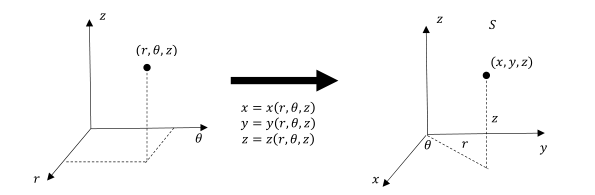
\includegraphics[scale=.75]{trans1}\end{center}
Show that 
\begin{align*}
x &= r\cos(\theta) \\
y &= r\sin(\theta) \\
z &= z
\end{align*}
and compute $\frac{\p(x,y,z)}{\p (r,\theta,z)}$.
\item[b.] 
Consider the spherical coordinates as a transformation from $\rho, \phi, \theta$ into $x,y,z$ space.
\begin{center}
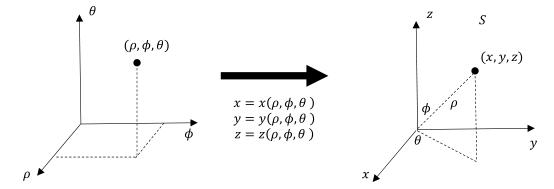
\includegraphics[scale=.75]{trans2}
\end{center}
Show that 
\begin{align*}
x &= \rho\sin(\phi)\cos(\theta)\\
y &= \rho\sin(\phi)\sin(\theta)\\
z &= \rho\cos(\phi)
\end{align*}
and compute $\frac{\p(x,y,z)}{\p(r,\phi,\theta)}$
\end{itemize}
\end{cproblem}
\begin{solution}
\vspace{-2em}
\begin{itemize}
\item[a.] By looking at the $x,y$ `floor' in the figure above, it is clear through basic trigonometry properties that $x = r\cos(\theta)$ and that $y = r\sin(\theta)$. Since the $z$ coordinate never changes between both transformations, $z=z$. Therefore the transformation is
\begin{align*}
x &= r\cos(\theta) \\
y &= r\sin(\theta) \\
z &= z
\end{align*}
Using this transformation I can compute
$$\frac{\p(x,y,z)}{\p(r,\theta,z)}= \Bigg| \bmat{\cos(\theta) & -r\sin(\theta) & 0 \\ \sin(\theta) & r\cos(\theta) & 0 \\ 0 & 0 & 1} \Bigg| = \left(r\cos^2(\theta)\right) + 0 + 0 - 0 - (-r\sin^2(\theta)) - 0 = r(\cos^2(\theta) + \sin^2(\theta)) = r.$$
\item[b.] The diagram above shows a point on the sphere in $x,y,z$ space with radius $\rho$. Using the diagram and trigonometry properties I see that the following is true
\begin{align*}
z &= \rho\cos(\phi) \\
r &= \rho\sin(\phi) 
\end{align*}
I can also describe the $(x,y,z)$ coordinate by using cylindrical coordinates. That is,
\begin{align*}
x &= r\cos(\theta) \\
y &= r\sin(\theta) \\
z &= z.
\end{align*}
Now, by substitution it is true that the parameterization of the (unit $\rho = 1$) sphere  is
\begin{align*}
x &= \rho\sin(\phi)\cos(\theta)\\
y &= \rho\sin(\phi)\sin(\theta)\\
z &= \rho\cos(\phi).
\end{align*}
The Jacobian is
$$\frac{\p(x,y,z)}{\p(\rho,\phi,\theta)} = \Bigg|\bmat{\sin(\phi)\cos(\theta) & \rho\cos(\phi)\cos(\theta) & -\rho\sin(\phi)\sin(\theta) \\ \sin(\phi)\sin(\theta) & \rho\cos(\phi)\sin(\theta) & \rho\sin(\phi)\cos(\theta) \\ \cos(\phi) & -\rho\sin(\phi) & 0}\Bigg|$$
and by the diagonalization method I get 
\begin{align*}
\frac{\p(x,y,z)}{\p(\rho,\phi,\theta)} = 0 &+ \left(\rho^2\cos^2(\phi)\cos^2(\theta)\sin(\phi)\right) + \left(\rho^2\sin^3(\phi)\sin^2(\theta)\right) \\ 
&- \left(-\rho^2\sin(\phi)\cos^2(\phi)\sin^2(\theta)\right) - 0 - \left(-\rho^2\sin^3(\phi)\cos^2(\theta) \right) \\
&= \rho^2\sin(\phi).
\end{align*}
\end{itemize}
\end{solution}

\begin{cproblem}{3}{White}
\ \\ \vspace{-2em}
\begin{itemize}
\item[a.] Consider a right circular cone of radius 10 meters and height 10 meters with a uniform density of $1\frac{kg}{m^3}$. Find the moment of inertia of this cone about its axis and use this to compute the kinetic energy of the cone spinning about its axis at a rate of $\omega\frac{radian}{second}$.
\item[b.] How long would it take (in minutes) for one horsepower motor generating $735\frac{newton\ meters}{sec}$ of power to accelerate this cone from rest to 1 revolution per second. [Ignore friction, air resistance, etc.]
\end{itemize}
\end{cproblem}
\begin{solution}
\begin{itemize}
\item[a.]The moment of inertia of a solid $S$ about its axis is defined as
$$\bigiiint{S}{} r^2\delta dV $$
Let the radius of the cone be $R = 10m$ and height $H = 10m$ and $\delta = 1$. Now, I want to describe a specific surface.
\begin{center} 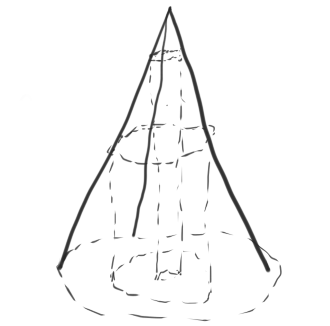
\includegraphics[scale=.5]{cone}\end{center}
Notice that the height of these cylinders are a function of the radius. So, let $z(r)$ be the height of a cylinder given the radius inside this cone. Notice when the height, $z(r)$, is infinitesimally small, the cylinder is an infinitely thin disk that is at $H$ with radius $R$ and when $z(r)= H$, the cylinder is an infinitely small disk at 0. Now, when $r = 0$, $z(r) = H$ and when $r = R$, $z(r) = 0$. So, to model this, it seems like $z(r) = H(1-\frac{r}{R}) = 10(1-\frac{r}{10}) = 10-r$. Now to describe this region, I can define $R = \{(r,\theta,z) \ | \ 0 \leq r \leq 10, \ 0\leq \theta\leq 2\pi, \ 0\leq z\leq z(r)\}$. $dV$ can be defined as $dV = rd\theta dzdr$ by the use of cylindrical coordinates. So, the moment of inertia becomes
$$\bigiiint{R}{}r^3d\theta dzdr = \mlvarint\limits_{0}^{10}\mlvarint\limits_{0}^{z(r)}\left[\mlvarint\limits_{0}^{2\pi}r^3 d\theta\right]dzdr = 2\pi\left(\frac{10^5}{4}-\frac{10^5}{5}\right) = 10000\pi(kg\cdot m).$$
Since I know that the moment of inertia is $10000\pi(kg\cdot m)$, and that kinetic energy is defined as $\frac{1}{2}I_s\omega^2$, I know that the kinetic energy of the cone spinning about the axis at a rate of $\omega\left(\frac{radians}{second}\right)$ is $\omega^25000\pi\left(\frac{kg\cdot m}{s^2}\right) = \omega^25000\pi (newton\cdot m)$
\item[b.] I know that $K.E = \omega^2 5000\pi$ and that $\omega = 1\left(\frac{rev}{sec}\right) = 2\pi \left(\frac{rad}{sec}\right)$. So, by substitution, 
$K.E = 4\pi^35000 (newton\cdot meter)$. Using the fact that $power = \frac{K.E}{T(sec)}$ I get that 
$$735\left(newton\cdot meter\right) = \frac{4\pi^3 5000}{T}\left(\frac{newton\cdot meter}{sec}\right)$$   
and solving for $T$ I get
$$T =  \frac{4\pi^35000}{735} (sec) = \frac{4\pi^35000}{735\cdot60}(min)$$
\end{itemize}
\end{solution}

\begin{cproblem}{4}{White}
Compute the moment of intertia about the $z$ axis of the following objects with uniform density $\delta$.
\begin{itemize}
\item[a.] The sphere $x^2 + y^2 + z^2 \leq a^2$
\item[b.] The cylinder $x^2 + y^2 \leq a^2, \ 0 \leq z\leq h$
\end{itemize}
\end{cproblem}
\begin{solution}
\vspace{-2em}
\begin{itemize}
\item[a.] I know that moment of inertia of a solid $S$ about its axis is defined as 
$$\bigiiint{S}{} r^2\delta dV $$
In this case $r^2 = (x^2 + y^2)$ and $dV = dxdydz$. So, I get that
$$\delta\bigiiint{S}{} (x^2 + y^2) dxdydz $$
and converting into spherical coordinates I get that $x^2 + y^2  = \rho^2\sin^2(\phi)$ and $dV = \frac{\p (x,y,z)}{\p (\rho,\phi,\theta)}$ which was calculated previously to be $dV = \frac{\p (x,y,z)}{\p (\rho,\phi,\theta)} = \rho^2\sin(\phi)$. By substitution I get the moment of inertia to be
$$\delta\bigiiint{R}{} (\rho^2\sin^2(\phi))\rho^2\sin(\phi) d\rho d\phi d\theta.$$
where $R = \{(\rho,\phi,\theta) \ | \ 0 \leq \rho \leq a, \ 0 \leq \phi \leq \pi, \ 0 \leq \theta \leq 2\pi\}$. So, 
$$\delta \mlvarint\limits_{0}^{2\pi}  \mlvarint\limits_{0}^{\pi}  \left[\mlvarint\limits_{0}^{a} (\rho^2\sin^2(\phi))\rho^2\sin(\phi) d\rho \right]d\phi d\theta = \frac{8\pi a^5\delta}{15}.$$
\item[b.] I know that moment of inertia of a solid $S$ about its axis is defined as 
$$\bigiiint{S}{} r^2\delta dV $$
Converting into cylindrical coordinates, $dV = \frac{\p(x,y,z)}{\p(r,\theta,z)} = r dr d\theta dz$ and $S$ becomes $R = \{(r,\theta,z) \ | \ 0 \leq r \leq a, \ 0 \leq \theta \leq 2\pi, \ 0 \leq z \leq h\}$. So, by substitution I get that the moment of inertia is
$$\delta \mlvarint\limits_{0}^{h} \mlvarint\limits_{0}^{2\pi} \left[ \mlvarint\limits_{0}^{a} r^3 dr\right]d\theta dz = \frac{\pi ha^4\delta}{2}.$$
\end{itemize}
\end{solution}

\begin{cproblem}{5}{White}
Since the only force we are considering is due to gravity, show that the potential energy at the top of the ramp is given by $mgh$ and use the result of that problem to show that the linear speed at the bottom of the ramp satasfies
$$ v^2 = \frac{2gh}{1+\frac{I}{ma^2}}$$
What is the velocity of each of the three objects in problem \#4 at the bottom of the ramp? Who wins the race? How does this compare to your guess at the beginning?
\end{cproblem}
\begin{solution}
By the conservation of energy, I know that the potential energy plus the kinetic energy equals some constant. I also know that at the bottom of the hill the potential energy of each object is zero and at the top of the hill the kinetic energy of each object is zero. This means that the kinetic energy at the bottom of the hill is equal to potential energy at the top of the hill. That means that,
$$ mhg = \frac{1}{2}m(1 + \frac{I}{ma^2})v^2 \implies 2gh = (1+\frac{I}{ma^2})v^2 \implies v^2 = \frac{2gh}{1+\frac{I}{ma^2}}.$$
Using this equation for the velocity of an object at the bottom of the hill, I can deduce that
\begin{align*}
v^2_c &= \frac{2gh}{1+\frac{I_c}{ma^2}} = \frac{2gh}{1+\frac{\pi ha^4\delta}{2(\delta\pi a^2 h)a^2}} = \frac{2gh}{1+\frac{1}{2}} = \frac{4}{3}gh\\
v^2_s &=  \frac{2gh}{1+\frac{I_s}{ma^2}} = \frac{2gh}{1 + \frac{4\cdot8\pi a^5\delta}{3\cdot15 \pi a^3 \delta a^2}} = \frac{10}{7}gh \\
v^2_{s_s} &=  \frac{2gh}{1+\frac{I{_s}_s}{ma^2}} = \frac{10}{7} gh
\end{align*}
Since there is no deceleration in any of the objects and $ v^2_c = \frac{4}{3}gh < \frac{7}{10}gh = v^2_s = v^2_{s_s}$, the two spheres touch the bottom at a tie and the cylinder drags behind. In comparison to my initial guess I was simply wrong!
\end{solution}
\end{document}